\documentclass{InsightArticle}

\usepackage[dvips]{graphicx}

%%%%%%%%%%%%%%%%%%%%%%%%%%%%%%%%%%%%%%%%%%%%%%%%%%%%%%%%%%%%%%%%%%
%
%  hyperref should be the last package to be loaded.
%
%%%%%%%%%%%%%%%%%%%%%%%%%%%%%%%%%%%%%%%%%%%%%%%%%%%%%%%%%%%%%%%%%%
\usepackage[dvips,
bookmarks,
bookmarksopen,
backref,
colorlinks,linkcolor={blue},citecolor={blue},urlcolor={blue},
]{hyperref}

\title{Computed Tomography Phantom Segmentation Results}

\release{1.00}

\author{Karthik Krishnan, Luis Ibanez, Wes Turner, Harvey Cline, Rick Avila}
\authoraddress{Kitware Inc., Clifton Park, NY}

\date{\today}

\begin{document}

\ifpdf
\else
   %
   % Commands for including Graphics when using latex
   % 
   \DeclareGraphicsExtensions{.eps,.jpg,.gif,.tiff,.bmp,.png}
   \DeclareGraphicsRule{.jpg}{eps}{.jpg.bb}{`convert #1 eps:-}
   \DeclareGraphicsRule{.gif}{eps}{.gif.bb}{`convert #1 eps:-}
   \DeclareGraphicsRule{.tiff}{eps}{.tiff.bb}{`convert #1 eps:-}
   \DeclareGraphicsRule{.bmp}{eps}{.bmp.bb}{`convert #1 eps:-}
   \DeclareGraphicsRule{.png}{eps}{.png.bb}{`convert #1 eps:-}
\fi


\newcommand{\composeFigureFromDatasetFeatures}[2]{

\subsubsection{Feature Generator Results for Dataset #1 #2}

\begin{figure}
\center
\includegraphics[width=1.0\textwidth]{GMSFG_Test#1_#2.png}
\itkcaption[Dataset #1 Gradient Magnitude Sigmoid Feature]{Dataset #1 #2 Results of Gradient Magnitude Sigmoid Feature Generator.}
\label{fig:Dataset#1#2GMSFG}
\end{figure}
\clearpage

\begin{figure}
\center
\includegraphics[width=1.0\textwidth]{SFG_Test#1_#2.png}
\itkcaption[Dataset #1 #2 Sigmoid Feature]{Dataset #1 #2 Results of Sigmoid Feature Generator.}
\label{fig:Dataset#1#2SFG}
\end{figure}
\clearpage

\begin{figure}
\center
\includegraphics[width=1.0\textwidth]{LWFG_Test#1_#2.png}
\itkcaption[Dataset #1 #2 Lung Wall Feature]{Dataset #1 #2 Results of Lung Wall Feature Generator.}
\label{fig:Dataset#1#2LWFG}
\end{figure}
\clearpage

\begin{figure}
\center
\includegraphics[width=1.0\textwidth]{MOFG_Test#1_#2.png}
\itkcaption[Dataset #1 #2 Morphological Openning Feature]{Dataset #1 #2 Results of Morphological Openning Feature Generator.}
\label{fig:Dataset#1#2MOFG}
\end{figure}
\clearpage

\begin{figure}
\center
\includegraphics[width=1.0\textwidth]{SVFG_Test#1_#2.png}
\itkcaption[Dataset #1 #2 Sato Vesselness Feature]{Dataset #1 #2 Results of Sato Vesselness Feature Generator.}
\label{fig:Dataset#1#2SVFG}
\end{figure}
\clearpage

\begin{figure}
\center
\includegraphics[width=1.0\textwidth]{SVSFG_Test#1_#2.png}
\itkcaption[Dataset #1 #2 Sato Vesselness Sigmoid Feature]{Dataset #1 #2 Results of Sato Vesselness Sigmoid Feature Generator.}
\label{fig:Dataset#1#2SVSFG}
\end{figure}
\clearpage

\begin{figure}
\center
\includegraphics[width=1.0\textwidth]{SLSFG_Test#1_#2.png}
\itkcaption[Dataset #1 #2 Sato Local Structure Feature]{Dataset #1 #2 Results of Sato Local Structure Feature Generator.}
\label{fig:Dataset#1#2SLSFG}
\end{figure}
\clearpage

\begin{figure}
\center
\includegraphics[width=1.0\textwidth]{DSFG_Test#1_#2.png}
\itkcaption[Dataset #1 #2 Descoteaux Sheetness Feature]{Dataset #1 #2 Results of Descoteaux Sheetness Feature Generator.}
\label{fig:Dataset#1#2DSFG}
\end{figure}
\clearpage

\begin{figure}
\center
\includegraphics[width=1.0\textwidth]{FTFG_Test#1_#2.png}
\itkcaption[Dataset #1 #2 Frangi Tubularness Feature]{Dataset #1 #2 Results of Frangi Tubularness Feature Generator.}
\label{fig:Dataset#1#2FTFG}
\end{figure}
\clearpage

\begin{figure}
\center
\includegraphics[width=1.0\textwidth]{SCRN_AFG_#1_#2.png}
\itkcaption[Dataset #1 #2 Features]{Dataset #1 #2 Results of Feature Generators.}
\label{fig:Dataset#1#2Features}
\end{figure}
\clearpage
}

\newcommand{\composeFigureFromDatasetSegmentations}[2]{

\subsubsection{Segmentation Results for Dataset #1 #2}

\begin{figure}
\center
\includegraphics[width=1.0\textwidth]{LSMT3_Test#1_#2.png}
\itkcaption[Dataset #1 #2 Segmentation Method 3]{Dataset #1 #2 Results of Segmentation Method 3.}
\label{fig:Dataset#1#2LSMT3}
\end{figure}
\clearpage

\begin{figure}
\center
\includegraphics[width=1.0\textwidth]{LSMT4_Test#1_#2.png}
\itkcaption[Dataset #1 #2 Segmentation Method 4]{Dataset #1 #2 Results of Segmentation Method 4.}
\label{fig:Dataset#1#2LSMT4}
\end{figure}
\clearpage

\begin{figure}
\center
\includegraphics[width=1.0\textwidth]{LSMT5_Test#1_#2.png}
\itkcaption[Dataset #1 #2 Segmentation Method 5]{Dataset #1 #2 Results of Segmentation Method 5.}
\label{fig:Dataset#1#2LSMT5}
\end{figure}
\clearpage

\begin{figure}
\center
\includegraphics[width=1.0\textwidth]{LSMT6_Test#1_#2.png}
\itkcaption[Dataset #1 #2 Segmentation Method 6]{Dataset #1 #2 Results of Segmentation Method 6.}
\label{fig:Dataset#1#2LSMT6}
\end{figure}
\clearpage

\begin{figure}
\center
\includegraphics[width=1.0\textwidth]{LSMT7_Test#1_#2.png}
\itkcaption[Dataset #1 #2 Segmentation Method 7]{Dataset #1 #2 Results of Segmentation Method 7.}
\label{fig:Dataset#1#2LSMT7}
\end{figure}
\clearpage

\begin{figure}
\center
\includegraphics[width=1.0\textwidth]{LSMT8_Test#1_#2.png}
\itkcaption[Dataset #1 #2 Segmentation Method 8]{Dataset #1 #2 Results of Segmentation Method 8.}
\label{fig:Dataset#1#2LSMT8}
\end{figure}
\clearpage

\begin{figure}
\center
\includegraphics[width=1.0\textwidth]{LSMT9_Test#1_#2.png}
\itkcaption[Dataset #1 #2 Segmentation Method 9]{Dataset #1 #2 Results of Segmentation Method 9.}
\label{fig:Dataset#1#2LSMT9}
\end{figure}
\clearpage

\begin{figure}
\center
\includegraphics[width=1.0\textwidth]{SCRN_ALSM_#1_#2.png}
\itkcaption[Dataset #1 #2 Segmentations]{Dataset #1 #2 Results of Segmentations.}
\label{fig:Dataset#1Segmentations}
\end{figure}
\clearpage
}

\newcommand{\insertResultsForDataset}[2]{
\subsection{Dataset #1 #2}
\composeFigureFromDatasetFeatures{#1}{#2}
\composeFigureFromDatasetSegmentations{#1}{#2}
}

\newcommand{\insertResultsForStack}[1]{
\insertResultsForDataset{#1}{001}
\insertResultsForDataset{#1}{002}
\insertResultsForDataset{#1}{003}
\insertResultsForDataset{#1}{004}
\insertResultsForDataset{#1}{005}
\insertResultsForDataset{#1}{006}
\insertResultsForDataset{#1}{007}
\insertResultsForDataset{#1}{008}
\insertResultsForDataset{#1}{009}
\insertResultsForDataset{#1}{010}
\insertResultsForDataset{#1}{011}
\insertResultsForDataset{#1}{012}
\insertResultsForDataset{#1}{013}
\insertResultsForDataset{#1}{014}
\insertResultsForDataset{#1}{015}
\insertResultsForDataset{#1}{016}
\insertResultsForDataset{#1}{017}
\insertResultsForDataset{#1}{018}
}

\maketitle

\ifhtml
\chapter*{Front Matter\label{front}}
\fi


\begin{abstract}
\noindent
This document summarizes the results of lung lesion segmentation methods
applied to a tomography phantom developed at NIST. In particular, this report
focuses on evaluating the precision of volume estimation by relying on the
known values of high precision beads that were incorporated into a phantom and
later CT scanned.

The figures presented in this report are generated by running the testing suite
over the dataset collection, and therefore should be reproducible in any
computer that has access to that collection.
\end{abstract}

\tableofcontents

\section{Introduction}

This report presents the results of applying the algorithm to a collection of
datasets. The results are presented both as a visual rendering of the resulting
segmentations and by providing quantitative estimations of lesion volume.

The phantom dataset included the following documentation:

\begin{verbatim}
3 November 2008

	This data was imaged by David Yankelevitz at the Weill Medical
School of Cornell University in the summer of 2008 (the date in the data
is not correct).  The images are of a set of 14 large pocket phantoms built
by Zachary Levine of NIST.  Each pocket phantom has six layers of 3 PTFE
balls in each layer.  These are Grade 1 balls with a manufacturer's
specification of 0.001" = 25 um.  The nominal diameters are 7/32", 1/4",
9/32", and 5/16", or 5.556 mm, 6.350 mm, 7.144 mm, and 7.938 mm,
respectively.  The diameters of the balls in each layer are the
same.   Twelve of the structures have an alternating pattern of 7/32"
and 5/16" (NIST-DP-A001 to NIST-DP-A012).  Two of the structure have an
alternative pattern of 1/4" and 9/32" (NIST-DP-B001 and NIST-DP-B002).

	The phantoms were wrapped in bubble wrap and placed in plastic
boxes with cardboard sleeves.  The images were made without unwrapping
the structures.

	The file LevineJResNIST2008b.pdf is to be published in J. Res.
Natl. Inst. Stand. and Technol. in November/December 2008.  This
describes a similar phantom with only one level.
\end{verbatim}

Therefore, when analyzing the results in this report, it is important to keep
in mind that the following sphere diameters where present in the phantom

\begin{itemize}
\item 5.556 mm
\item 6.350 mm
\item 7.144 mm
\item 7.938 mm
\end{itemize}

The types of beads are paired in two types of stacks.

\begin{itemize}
\item Stack A: contains beads of diameters
\begin{itemize}
\item 5.556 mm
\item 7.938 mm
\end{itemize}
\item Stack B: contains beads of diameters
\begin{itemize}
\item 6.350 mm
\item 7.144 mm
\end{itemize}
\end{itemize}

When evaluating precision of the segmentations we will verify that every bead
is compared to the appropriate base value from the list above.

Figure~\ref{fig:GlobalView} shows a slice of the phantom, where the 14 plastic
boxes storing the LEGO stacks are visible.

\begin{figure}
\center
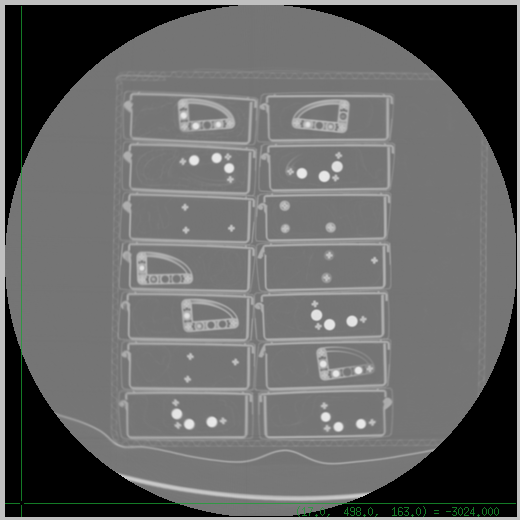
\includegraphics[width=1.0\textwidth]{NIST_A.png}
\itkcaption[Global View of the Phantom]{Global View of the NIST Phantom}
\label{fig:GlobalView}
\end{figure}
\clearpage

\begin{figure}
\center
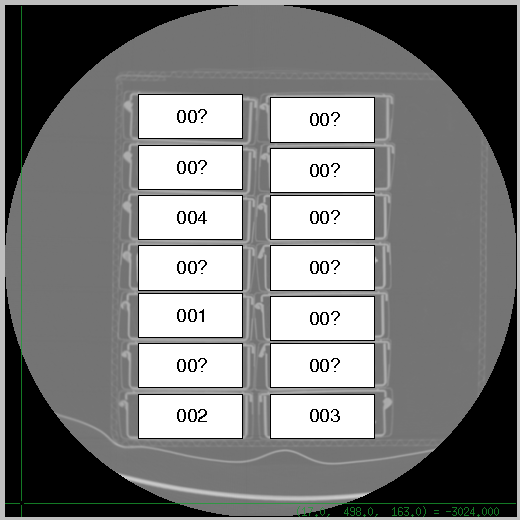
\includegraphics[width=1.0\textwidth]{NIST_A_Catalog.png}
\itkcaption[Catalog of Stacks]{Catalog of stacks in the global view of the NIST Phantom}
\label{fig:StackCatalog}
\end{figure}
\clearpage


\section{Algorithm Description}

\section{Segmentation Results Visualizations}

%\insertResultsForStack{NIST001}
%\insertResultsForStack{NIST002}
%\insertResultsForStack{NIST003}
%\insertResultsForStack{NIST004}

\small
\listoffigures
\listoftables
\normalsize

\end{document}

